\documentclass{article}
\usepackage{iclr2027_conference,times}
\usepackage{amsmath,amssymb,amsthm,booktabs,graphicx,xcolor,tikz}
\usepackage{hyperref}
\usepackage{url}

\newtheorem{proposition}{Proposition}
\newcommand{\E}{\mathbb{E}}
\newcommand{\Var}{\operatorname{Var}}
\newcommand{\sg}{\operatorname{sg}}
\newcommand{\clip}{\operatorname{clip}}
\newcommand{\todo}[1]{\textcolor{red!70!black}{\textbf{[TODO: #1]}}}
\definecolor{baselinecurve}{HTML}{365B88}
\definecolor{regcurve}{HTML}{A64920}
\makeatletter
\newcommand{\tablerows}[1]{\@@input #1 }
\makeatother

\title{Regularizing Cumulative Importance Weights in Sequential Multi-Agent Policy Optimization}
\author{Anonymous authors}
% TODO: Confirm author list and affiliations for a non-anonymous version.
% \iclrfinalcopy

\begin{document}
\maketitle

\begin{abstract}
Sequential policy updates let cooperative agents adapt to teammates as their policies change. Heterogeneous-agent proximal policy optimization (HAPPO) implements this approach by reusing a shared rollout and multiplying importance ratios to account for agents that have already updated. The variance of this cumulative weight can grow exponentially with the number of preceding agents, amplifying gradient noise and making later updates less stable. We propose Reg-HAPPO, which adds a penalty for the squared change in the cumulative weight induced by each policy update. This penalty discourages large changes on transitions where the preceding agents have already produced large weights. Under conditionally factorized policies and a fixed rollout context distribution, we show that the expected squared change equals the increment in importance-weight variance and characterize it through order-two R\'enyi divergence. Compared with HAPPO, Reg-HAPPO increases mean win rates in cooperative micromanagement and yields more consistent performance across training seeds in several benchmark settings.
\end{abstract}

\section{Introduction}

\section{Related work}

\paragraph{Trust-region methods for cooperative learning.}
Trust Region Policy Optimization (TRPO) constrains the Kullback--Leibler (KL) divergence between successive policies, while Proximal Policy Optimization (PPO) can limit changes through a clipped surrogate objective~\citep{schulman2015,schulman2017}. Multi-Agent PPO (MAPPO) uses a centralized value function to train decentralized policies with per-agent PPO ratios~\citep{yu2022}. Heterogeneous-Agent TRPO (HATRPO) and Heterogeneous-Agent PPO (HAPPO) use advantage decomposition to update policies sequentially. They reuse the rollout collected before the sequence of updates and apply importance sampling to account for teammates that have already updated~\citep{kuba2022}. \citet{zhong2024} extend this sequential framework to a broader class of algorithms through heterogeneous-agent mirror learning. \citet{shek2026} allocate a joint KL budget across HATRPO updates. The Multi-Agent Transformer (MAT) uses the advantage decomposition to parameterize a policy that conditions each action on preceding agents' actions~\citep{wen2022}. We study sequential policy updates with conditionally independent action sampling.

\paragraph{Variance from teammates' policy updates.}
\citet{kuba2021variance} analyze how policy-gradient baselines can reduce variance due to teammates' exploration. A separate source of variance comes from multiplying teammates' likelihood ratios when their policies change on a shared batch~\citep{wu2021,le2025}. Coordinated PPO (CoPPO) clips the product of other agents' ratios before applying a second clipping operation to the combined ratio~\citep{wu2021}. Agent-by-agent Policy Optimization (A2PO) uses a Retrace-inspired correction to estimate advantages under policies in which preceding agents have updated~\citep{wang2023}. \citet{le2025} show that the variance of the prefix weight can grow exponentially with the number of preceding agents and cap this weight in the surrogate for clip-HAPPO and clip-HATRPO. \citet{zhao2026aggregate} study products of agents' ratios in jointly differentiated objectives and propose aggregating information in the advantage. Reg-HAPPO uses the original prefix weight in HAPPO's surrogate and penalizes the squared change in the cumulative weight caused by the current policy update. The same change in the current agent's ratio incurs a larger penalty on samples with larger prefix weights.

\paragraph{R\'enyi divergence in importance sampling.}
Policy Optimization via Importance Sampling (POIS) uses a R\'enyi-divergence term in a high-confidence surrogate for reusing trajectories in single-agent policy search~\citep{metelli2018,metelli2020}. In action-based POIS, trajectory likelihood ratios accumulate over time. Reg-HAPPO uses the same relation between order-two R\'enyi divergence and importance-weight variance for a product over agents at a single transition. For valid cumulative importance weights with finite variance, conditional factorization and a fixed rollout context distribution make the expected squared change in the cumulative weight equal to the variance increment attributable to the current agent's update.


\section{Preliminaries}

\subsection{Problem formulation}
\label{sec:problem-formulation}

We model fully cooperative multi-agent reinforcement learning as a partially observable Markov game~\citep{littman1994,bernstein2002}. At time $t$, the environment is in state $s_t\in\mathcal S$, and each agent $i\in\mathcal N=\{1,\ldots,n\}$ receives a local observation $o_t^i\in\mathcal O^i$ and simultaneously selects an action $a_t^i\in\mathcal A^i$. Given $s_t$ and the joint action $\boldsymbol a_t=(a_t^1,\ldots,a_t^n)$, the team receives a shared bounded reward $R(s_t,\boldsymbol a_t)$ and the environment draws the next state from $P(\cdot\mid s_t,\boldsymbol a_t)$ and the next joint observation from $Z(\cdot\mid s_{t+1},\boldsymbol a_t)$. Starting from an initial state and observation distribution $\mu_0$, the team seeks a joint policy $\pi$ that maximizes $J(\pi)=\E_\pi[G_0]$, where $G_t=\sum_{k=0}^{\infty}\gamma^k R(s_{t+k},\boldsymbol a_{t+k})$ and $\gamma\in[0,1)$.

\subsection{Sequential policy updates in HAPPO}
\label{sec:happo}

Following HAPPO~\citep{kuba2022}, we write each actor's policy as a function of the state $s$ with separate parameters $\theta_i$. For observation-based actors, we include the current joint observation in $s$ and evaluate each actor on its local observation $o^i$. With independent action sampling given $s$, the joint policy factorizes as
\begin{equation}
    \pi_{\boldsymbol\theta}(\boldsymbol a\mid s)
    =\prod_{i\in\mathcal N}\pi_{\theta_i}^i(a^i\mid s).
    \label{eq:factorized-joint-policy}
\end{equation}

HAPPO draws a random update order each iteration, and we index agents by their position in that order. When agent $i$ updates, each agent $j<i$ already has new parameters $\theta_j^+$. The surrogate evaluates the update with these new teammate policies and uses the old-policy advantage $A_{\pi_{\mathrm{old}}}$ as a fixed reference~\citep{kuba2022}. Since the rollout was collected under $\pi_{\mathrm{old}}$, HAPPO reweights the sampled actions by importance sampling. For policies supported by their rollout counterparts, define
\begin{equation}
    r_j(\theta_j)=\frac{\pi_{\theta_j}^{j}(a^{j}\mid s)}
                        {\pi_{\mathrm{old}}^{j}(a^{j}\mid s)},
    \qquad W_{i-1}=\prod_{j<i}r_j(\theta_j^{+}), \qquad W_0=1.
    \label{eq:happo-importance-weights}
\end{equation}
The prefix weight $W_{i-1}$ changes the action distribution of agents $j<i$ at the sampled state $s$. It stays fixed during agent $i$'s update, while $r_i(\theta_i)$ changes with its policy. Once that update is complete, the next agent uses $W_i=W_{i-1}r_i(\theta_i^+)$.

Write $\E_{\mathrm{old}}$ for expectation under the rollout distribution, with state marginal $d_{\mathrm{old}}$. The joint advantage is $A_{\pi}=Q_{\pi}-V_{\pi}$, where $Q_{\pi}$ and $V_{\pi}$ are the expected remaining returns given $(s,\boldsymbol a)$ and $s$, respectively. Advantage decomposition gives the marginal surrogate $\E_{\mathrm{old}}[W_{i-1}(r_i(\theta_i)-1)A_{\pi_{\mathrm{old}}}]$~\citep{kuba2022}. Using an estimate $\hat A$ of the old-policy advantage, HAPPO maximizes the clipped objective~\citep{kuba2022,schulman2017}
\begin{equation}
    \mathcal L_{\mathrm{HAPPO}}^i(\theta_i)
    =\E_{\mathrm{old}}\!\left[
      W_{i-1}\min\!\left\{
        r_i(\theta_i)\hat A,\,
        \clip(r_i(\theta_i),1-\epsilon,1+\epsilon)\hat A
      \right\}
    \right],
    \label{eq:happo-surrogate}
\end{equation}
where $\epsilon>0$ is the clipping threshold for $r_i$.

\subsection{Variance from prefix importance weights}
\label{sec:prefix-weight-variance}

For fixed old and updated policies, each preceding ratio has mean one when actions are sampled from the rollout policy at a given state $s$. Write $v_j(s)=\Var_{\mathrm{old}}(r_j(\theta_j^+)\mid s)$ for the variance of agent $j$'s ratio. By conditional independence, the prefix weight also has mean one and its variance is
\begin{equation}
    \Var_{\mathrm{old}}(W_{i-1}\mid s)=\prod_{j<i}\bigl(1+v_j(s)\bigr)-1.
    \label{eq:prefix-weight-variance}
\end{equation}
If every preceding ratio has variance at least $\delta>0$ at $s$, the prefix variance grows at least as $(1+\delta)^{i-1}-1$. A large prefix weight amplifies a sample's contribution to the policy gradient even at the start of agent $i$'s update, when $r_i=1$ and clipping is inactive.

\paragraph{A one-step switch game.}
Each agent simultaneously sets one switch to $a^i\in\{-1,+1\}$. The episode ends with a shared reward equal to the average switch value, $R(\boldsymbol a)=n^{-1}\sum_{i=1}^n a^i$ (Fig.~\ref{fig:switch-game}a). The rollout policy sets each switch uniformly and independently, so the exact old-policy advantage is $R(\boldsymbol a)$. In each update, we move the probability of $+1$ from $1/2$ to $(1+\epsilon)/2$ for $0<\epsilon<1$. This maximizes the concave surrogate in Eq.~\eqref{eq:happo-surrogate}, which increases up to the upper clipping boundary and has nonpositive slope above it. Each preceding ratio is then $1+\epsilon a^j$ and has variance $\epsilon^2$.

At the start of update $i$, the single-sample gradient with respect to agent $i$'s Bernoulli logit is $g_i=W_{i-1}R(\boldsymbol a)a^i/2$. Averaging over the current switch with all others fixed gives $W_{i-1}/(2n)$, so the expected gradient is $1/(2n)$ at every position. The variance of this conditional average alone gives a lower bound on the gradient variance
\begin{equation}
    \Var_{\mathrm{old}}(g_i)
    \ge \frac{\Var_{\mathrm{old}}(W_{i-1})}{4n^2}
    = \frac{(1+\epsilon^2)^{i-1}-1}{4n^2}.
    \label{eq:switch-game-variance}
\end{equation}
For eight agents and $\epsilon=0.5$, the gradient variance rises from $0.0273$ at the first update to $0.646$ at the last (Fig.~\ref{fig:switch-game}b). This motivates controlling how much variance each update adds to the prefix weight passed to later agents.

\begin{figure}[tb]
    \centering
    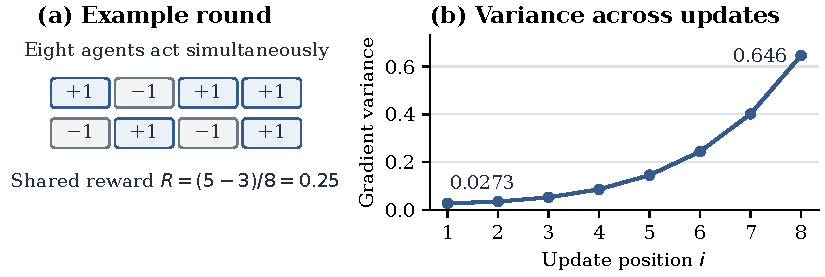
\includegraphics[width=\linewidth]{figures/switch_game_variance.pdf}
    \caption{The one-step switch game. (a) Eight agents choose their switches simultaneously and share the mean switch value as reward. (b) Exact variance of the single-sample logit gradient at the start of each update, from all $2^8$ equally likely joint actions under the rollout policy. With $\epsilon=0.5$, each completed update changes the probability of $+1$ from $0.50$ to $0.75$. The expected gradient stays at $1/16$, while the last update has $23.6$ times the variance of the first.}
    \label{fig:switch-game}
\end{figure}

\section{Method}


\section{Experiments}


\section{Conclusion}

\bibliography{references}
\bibliographystyle{iclr2027_conference}

\appendix
\section{details}

\end{document}
